\documentclass{../../commons/assignment}

\usepackage{float}
\usepackage{tikz}
\usepackage{adjustbox}
\usepackage{titlesec}
\usepackage{soul}
\usepackage{csvsimple}

\usepackage{pgfplots}
\usepackage{graphics, epsfig}

\usepackage{graphicx}
\usepackage{subcaption}

\usetikzlibrary{decorations.pathmorphing, decorations.markings}
\usetikzlibrary{positioning}

\usetikzlibrary{calc,patterns,angles,quotes}
\setlength{\parindent}{0pt}

\usetikzlibrary{shapes, arrows}
\tikzstyle{startstop} = [rectangle, rounded corners, minimum width=3cm, minimum height=1cm, text centered, draw=black, fill=red!30]
\tikzstyle{io} = [trapezium, trapezium stretches=true, trapezium left angle=70, trapezium right angle=110, minimum width=4cm, minimum height=1cm, text centered, draw=black, fill=blue!30]
\tikzstyle{process} = [rectangle, minimum width=4cm, minimum height=1cm, text centered, text width=4cm, draw=black, fill=orange!30]
\tikzstyle{decision} = [diamond, minimum width=3cm, minimum height=1cm, text centered, draw=black, fill=green!30]
\tikzstyle{arrow} = [thick,->,>=stealth]

\hypersetup{
pdftitle={ME621 - Advanced Finite Element Methods},
pdfsubject={Report for assignment 4},
pdfauthor={Tommaso Bocchietti}
}

\begin{document}
\graphicspath{{./img/}}


\title{ME621 - Advanced Finite Element Methods \\ Assignment 4}
\author{Tommaso Bocchietti}
\date{A.Y. 2023/24 - W24}

\maketitle

\begin{figure}[H]
    \centering
    
\includegraphics[width=.9\textwidth]{./pdf/UniversityOfWaterloo_logo_vert_pms.pdf}
    \label{fig:University_Of_Waterloo_logo}
\end{figure}

\clearpage
\tableofcontents
\listoffigures
\listoftables
\clearpage

\section{Requests}
\label{sec:requests}

A system of two aluminum bars of the same material is shown in the following figure.
The system is subjected to two external loads, $P_x$ and $P_y$, at joint B.
A and C are connected to pinned supports.

\begin{figure}[h]
    \centering
    \begin{tikzpicture}[scale=3]

        \coordinate (A) at (0,0.5);
        \coordinate (B) at (3,0.5);
        \coordinate (Bf) at (3.7,1);
        \coordinate (C) at (3,0);

        % Joint names
        \node at (A) [above, left] {A};
        \node at (B) [below, above] {B};
        \node at (C) [below, left] {C};

        % Initial position
        \draw (A) -- (B) node[midway, below] {$L_1$};
        \draw (C) -- (B) node[midway, left] {$L_2$};

        % Deformed position
        \draw[dashed] (A) -- (Bf)node[midway, above] {$l_1$};
        \draw[dashed] (C) -- (Bf)node[midway, right] {$l_2$};

        % Labels
        \pic [draw, ->, "$\alpha$", angle radius=2cm] {angle = B--A--Bf};
        \pic [draw, <-, "$\beta$", angle radius=0.7cm] {angle = Bf--C--B};

        % Support at the end of Beam 1
        \draw[fill] (0,0.5) circle (0.03);

        % Support at the end of Beam 2
        \draw[fill] (3,0) circle (0.03);

        % Arrows at coordinate Bf
        \draw[->] (Bf) -- ++(0.3, 0) node[right] {$\vec{P_x}$};
        \draw[->] (Bf) -- ++(0, 0.3) node[above] {$\vec{P_y}$};
        \draw[->] (B) -- (Bf) node[midway, above] {$\vec{u}$};
        % \draw[->, shorten >=150pt] (Bf) -- (A) node[above, above] {$\vec{F_1}$};
        % \draw[->, shorten >=50pt] (Bf) -- (C) node[above, right] {$\vec{F_2}$};

    \end{tikzpicture}
    \caption{Problem representation}
    \label{fig:problem_representation}
\end{figure}

The problem asks to:

\begin{itemize}
    \item Obtain the external loads $P_x$ and $P_y$ as a function of horizontal and vertical displacements at point B (namely $u$ and $v$).
    \item Determine the displacements in both $x$ and $y$ directions for $1000$ load increments of $+5\text{N}$ for both $P_x$ and $P_y$ (from zero).
    \item Find the displacement of point B after the final increment.
\end{itemize}

Write a \texttt{MATLAB} code with a convergence error of $10^-5$ to numerically solve the problem.
Use a combination of (a) Euler and N-R, and (b) Euler and modified N-R.
Also plot the resultant force versus the resultant displacement.

Use the Green strain measure:

\begin{equation}
    E_i = \frac{l_i^2 - L^2}{2L^2}
    \label{eq:green_strain_measure_formula}
\end{equation}

From now on, we will refer to the Green strain measure as $\epsilon_{1,2}$ to differentiate it from the Young's modulus $E_{1,2}$.

\begin{table}[H]
    \centering
    \begin{tabular}{|c|c|c|}
        \hline
        \textbf{Parameter} & \textbf{Value} & \textbf{Unit} \\ \hline
        $E_1 = E_2 = E$    & $70$           & $\text{GPa}$  \\ \hline
        $L_1$              & $3$            & $\text{m}$    \\ \hline
        $L_2$              & $0.5$          & $\text{m}$    \\ \hline
        $A_1 = A_2 = A$    & $0.0001$       & $\text{m}^2$  \\ \hline
    \end{tabular}
    \caption{Parameters of the system}
    \label{tab:parameters_of_the_system}
\end{table}

\section{Methodology}
\label{sec:methodology}

We will start by writing the analytical expression of the \textbf{shape functions} for the 4-node element with total length $h_e$ and $\alpha = \beta = \frac{1}{3}$ in terms of the parent coordinate system, $-1 \leq \xi \leq 1$.
To do so, we will make use of \texttt{Mathematica} to perform the symbolic computation and obtain the exact expression of the shape functions.

We will proceed by writing the elemental matrices ($B_0^e$, $f_{int}^e$, $f_{ext}^e$, $f_{kin}^e$) still in terms of the parent coordinate system.

We will then write the \textbf{MATLAB} code to solve the problem implementing the explicit integration scheme with Total Lagrangian finite element formulation and finally plot the deformation of the right end of the bar vs time, namely $u_{end}(t)$.
\section{Solution}

\subsection{Equilibrium equations}

We can start writing the equilibrium equations for the system.
Since we have no data about the mass of the bars, we will assume negligible mass of the bars.
This assumption will allow us to neglect the effect of gravity on the system and avoid the introduction of the inertia terms in the equilibrium equations.

\begin{equation}
    % TODO: check equilibrium equations
    \vec{F_{ext}} + \vec{F_{int}} = \vec{0}
    \label{eq:equilibrium_equations_1}
\end{equation}

\begin{equation}
    \begin{cases}
        \vec{F_{ext}} = \vec{P_x} + \vec{P_y} \\
        \vec{F_{int}} = \vec{F_{int,x}} + \vec{F_{int,y}}
    \end{cases}
\end{equation}

By decomposing the equations in the $x$ and $y$ directions, we obtain:

\begin{equation}
    \begin{cases}
        P_x = F_{int,x} = |F_1|*\cos(\alpha) + |F_2|*\sin(\beta) \\
        P_y = F_{int,y} = |F_1|*\sin(\alpha) + |F_2|*\cos(\beta)
    \end{cases}
    \label{eq:equilibrium_equations_2}
\end{equation}
\subsection{Force displacement relationship}

So far we have obtained the equilibrium equations for the system.
We can now proceed to obtain the force displacement relationship, which will allow us to solve the system of equations ${\vec{P}} = f({\vec{u}})$.
To do so, we try to express everything on the right-hand side of the equilibrium equations in terms of the displacements $u$ and $v$.

From simple trigonometrical considerations, we can obtain the following relationships:

\begin{align}
    \cos(\alpha) & = \frac{\text{L}_1+u}{l_1} \\
    \sin(\alpha) & = \frac{v}{l_1}            \\
    \cos(\beta)  & = \frac{\text{L}_2+u}{l_2} \\
    \sin(\beta)  & = \frac{v}{l_2}
\end{align}

We can now proceed working on the forces, knowing that the internal forces are linked to the strains by the following relationship:

\begin{equation}
    \begin{Bmatrix}
        \vec{F_{int,x}} \\
        \vec{F_{int,y}}
    \end{Bmatrix}
    =
    \begin{Bmatrix}
        \text{A}_1 * \text{E}_1 * \epsilon_1 \\
        \text{A}_2 * \text{E}_2 * \epsilon_2
    \end{Bmatrix}
\end{equation}

And the strains are linked to the displacements by the following relationship:

\begin{equation}
    \begin{Bmatrix}
        \epsilon_1 \\
        \epsilon_2
    \end{Bmatrix}
    =
    \begin{Bmatrix}
        \frac{l_1^2-\text{L}_1^2}{2 \text{L}_1^2} \\
        \frac{l_2^2-\text{L}_2^2}{2 \text{L}_2^2}
    \end{Bmatrix}
\end{equation}

Finally, we can give the following definition to the real length of the bars:

\begin{equation}
    \begin{Bmatrix}
        l_1 \\
        l_2
    \end{Bmatrix}
    =
    \begin{Bmatrix}
        \sqrt{(\text{L}_1+u)^2+v^2} \\
        \sqrt{u^2+(\text{L}_2+v)^2}
    \end{Bmatrix}
\end{equation}

We can now substitute the equations above in the equilibrium equations \ref{eq:equilibrium_equations_2} to obtain the force displacement relationship:

\begin{equation}
    \begin{Bmatrix}
        \vec{P_x} \\
        \vec{P_y}
    \end{Bmatrix}
    =
    \begin{Bmatrix}
        \frac{\text{A}_1 \text{E}_1 (\text{L}_1+u) \left(-\text{L}_1^2+(\text{L}_1+u)^2+v^2\right)}{2 \text{L}_1^2 \sqrt{(\text{L}_1+u)^2+v^2}} + \frac{\text{A}_2 \text{E}_2 v \left(-\text{L}_2^2+u^2+(\text{L}_2+v)^2\right)}{2 \text{L}_2^2 \sqrt{u^2+(\text{L}_2+v)^2}} \\
        \frac{\text{A}_1 \text{E}_1 v \left(-\text{L}_1^2+(\text{L}_1+u)^2+v^2\right)}{2 \text{L}_1^2 \sqrt{(\text{L}_1+u)^2+v^2}} + \frac{\text{A}_2 \text{E}_2 (\text{L}_2+u) \left(-\text{L}_2^2+u^2+(\text{L}_2+v)^2\right)}{2 \text{L}_2^2 \sqrt{u^2+(\text{L}_2+v)^2}}
    \end{Bmatrix}
    \label{eq:force_displacement_relationship}
\end{equation}

Even if quite long, the equation \ref{eq:force_displacement_relationship} are nothing more than a function ${\vec{P}} = f({\vec{u}})$ which can be solved numerically for a given value of ${\vec{P*}}$ to find the corresponding value of ${\vec{u*}}$.

\subsection{Linearization}

Before proceeding with the numerical solution of the system, we can try to linearize the system of equations to obtain a linear system of equations.
To do so, we can use a Taylor series expansion of the force-displacement relationship \ref{eq:force_displacement_relationship} around the point $\vec{u} = \vec{0}$.
A general Taylor series expansion of a function $f(x, y)$ around the point $(x_0, y_0)$ is given by:

\begin{align}
    f(x, y) & = f(x_0, y_0) + \nonumber                                                                                                                                                                                                                                  \\
            & + \frac{\partial f}{\partial x}(x_0, y_0) \cdot (x - x_0) + \frac{\partial f}{\partial y}(x_0, y_0) \cdot (y - y_0) + \nonumber                                                                                                                            \\
            & + \frac{1}{2} \frac{\partial^2 f}{\partial x^2}(x_0, y_0) \cdot (x - x_0)^2 + \frac{1}{2} \frac{\partial^2 f}{\partial y^2}(x_0, y_0) \cdot (y - y_0)^2 + \frac{\partial^2 f}{\partial x \partial y}(x_0, y_0) \cdot (x - x_0) \cdot (y - y_0) + \nonumber \\
            & + \dots
\end{align}

We can now try to apply the (1° order) Taylor series expansion to the force-displacement relationship \ref{eq:force_displacement_relationship} to obtain the following system of linear equations:

We can now try to apply the Taylor series expansion to the force-displacement relationship \ref{eq:force_displacement_relationship}.


\subsubsection{Taylor series of order 1}

By applying the Taylor series expansion of order 1, we obtain the following system of linear equations:

\begin{equation}
    \begin{Bmatrix}
        \widehat{\vec{P_x}} \\
        \widehat{\vec{P_y}}
    \end{Bmatrix}
    =
    \begin{Bmatrix}
        \frac{\text{A}_1 \text{E}_1 u}{\text{L}_1} \\
        \frac{\text{A}_2 \text{E}_2 v}{\text{L}_2}
    \end{Bmatrix}
\end{equation}


\subsubsection{Taylor series of order 2}

By applying the Taylor series expansion of order 2, we obtain the following system of quadratic equations:

\begin{equation}
    \begin{Bmatrix}
        \widehat{\widehat{\vec{P_x}}} \\
        \widehat{\widehat{\vec{P_y}}}
    \end{Bmatrix}
    =
    \begin{Bmatrix}
        \frac{\text{A}_1 \text{E}_1 u}{\text{L}_1}+\frac{\text{A}_2 \text{E}_2 v^2}{\text{L}_2^2}+\frac{\text{A}_1 \text{E}_1 \left(u^2+v^2\right)}{2 \text{L}_1^2} \\
        \frac{\text{A}_2 \text{E}_2 v}{\text{L}_2}+\frac{\text{A}_1 \text{E}_1 uv}{\text{L}_1^2}+\frac{\text{A}_2 \text{E}_2 \left(u^2+2 u v-v^2\right)}{2 \text{L}_2^2}
    \end{Bmatrix}
\end{equation}


\subsubsection{Taylor series of order 3}

By applying the Taylor series expansion of order 3, we obtain the following system of cubic equations:

\begin{equation}
    \begin{Bmatrix}
        \widehat{\widehat{\widehat{\vec{P_x}}}} \\
        \widehat{\widehat{\widehat{\vec{P_y}}}}
    \end{Bmatrix}
    =
    \begin{Bmatrix}
        \frac{\text{A}_1 \text{E}_1 u}{\text{L}_1}+\frac{\text{A}_2 \text{E}_2 v^2}{\text{L}_2^2}-\frac{\text{A}_1 \text{E}_1 u v^2}{2 \text{L}_1^3}-\frac{\text{A}_2 \text{E}_2 v \left(-u^2+v^2\right)}{2 \text{L}_2^3}+\frac{\text{A}_1 \text{E}_1 \left(u^2+v^2\right)}{2 \text{L}_1^2} \\
        \frac{\text{A}_2 \text{E}_2 v}{\text{L}_2}+\frac{\text{A}_1 \text{E}_1 u v}{\text{L}_1^2}+\frac{\text{A}_2 \text{E}_2 \left(u^2+2 u v-v^2\right)}{2 \text{L}_2^2}+\frac{\text{A}_1 \text{E}_1 v \left(-u^2+v^2\right)}{2 \text{L}_1^3}+\frac{\text{A}_2 \text{E}_2 \left(u^3-2 u^2 v-u v^2+v^3\right)}{2 \text{L}_2^3}
    \end{Bmatrix}
\end{equation}


\subsubsection{Comparison}

As it's easy to understand, the system of equations obtained with the Taylor series expansion of order 2 (since it has a higher order) is more accurate than the system of equations obtained with the Taylor series expansion of order 1.
We can now compare the results obtained with the two systems of equations to understand the error introduced by the linearization.
In the following figures, we can see the error introduced by the linearization with respect to the original force-displacement relationship \ref{eq:force_displacement_relationship}.

\begin{figure}[H]
    \centering
    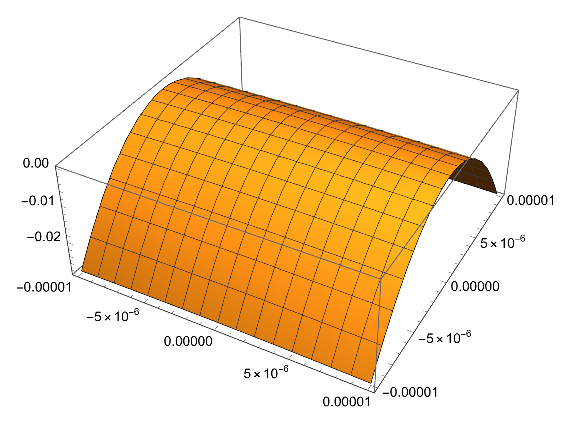
\includegraphics[width=.5\textwidth]{./pdf/residual_taylor_order_1}
    \caption{Error analysis for a Taylor series of order 1}
    \label{fig:residual_taylor_order_1}
\end{figure}

\begin{figure}[H]
    \centering
    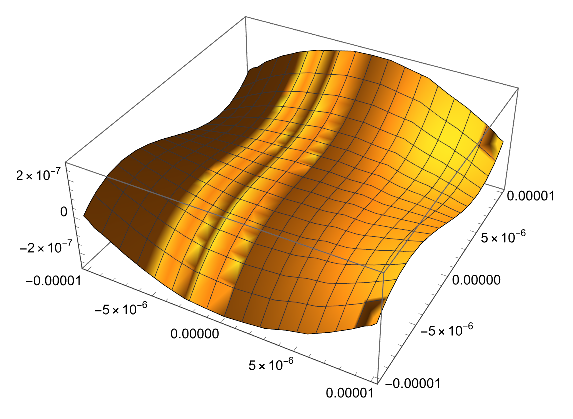
\includegraphics[width=.5\textwidth]{./pdf/residual_taylor_order_2}
    \caption{Error analysis for a Taylor series of order 2}
    \label{fig:residual_taylor_order_2}
\end{figure}

\begin{figure}[H]
    \centering
    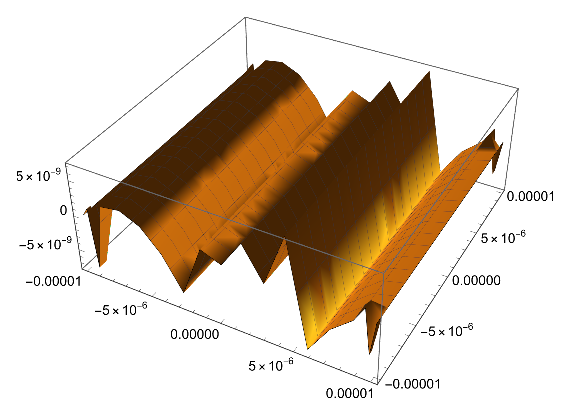
\includegraphics[width=.5\textwidth]{./pdf/residual_taylor_order_3}
    \caption{Error analysis for a Taylor series of order 3}
    \label{fig:residual_taylor_order_3}
\end{figure}

As we can see, around the point $\vec{u} = \vec{0}$, the error is negligible for both the approximations.
However, as we move away from the point $\vec{u} = \vec{0}$, the error introduced by the linearization increases.

In particular, we can see that the error introduced by the linearization decreases as we increase the order of the Taylor series expansion.

\section{Results}
\label{sec:results}

The numerical results for the problem described in Section \ref{sec:requests} are reported in the following.

When not specified, the results are obtained with the following boundary conditions imposed on the structure:

\begin{table}[H]
    \centering
    \begin{tabular}{|l|c|c|c|c|}
        \hline
        ~            & $U_x$ & $U_y$ & $V_x$ & $V_y$ \\
        ~            & m     & m     & m/s   & m/s   \\
        \hline
        Bottom nodes & Fixed & Fixed & 0     & 0     \\
        Top nodes    & -     & Fixed & 1     & 0     \\
        \hline
    \end{tabular}
    \caption{Boundary conditions imposed on the structure.}
    \label{tab:boundary_conditions}
\end{table}


\paragraph{Average $\sigma_{12}(\gamma)$ for element \#1}

To answer the first question of the assignment, we have decided to consider for the computation of the average shear stress $\sigma_{12}$ just the first element of the mesh, which is the one in the bottom-left corner of the structure.
Moreover, given that $\sigma_{12}$ get computed in every Gaussian point of the element, to simplify the computation, we have decided to consider just the Gaussian point in elemental coordinates $(\eta, \xi) = (-1/\sqrt{3}, -1/\sqrt{3})$, which is the one in the bottom-left corner of the element.
This choice is justified by the fact that $\gamma$, which is the shear strain of the element, is usually referred to the bottom-left corner of the element with the hypotheses of null gradient all over the element (i.e., $\gamma_{element} = \gamma_{bottom-left} \rightarrow \gamma(x, y) = \gamma(0, 0)$).

With the hypothesis of null or almost null $\nabla \gamma$ in the element, we report in Figure \ref{fig:shear_stress_vs_strain} the shear stress $\sigma_{12}$ as a function of the shear strain $\gamma$ until $\gamma = 0.07$.

\begin{figure}[H]
    \centering

    \begin{minipage}[b]{0.45\textwidth}
        \centering
        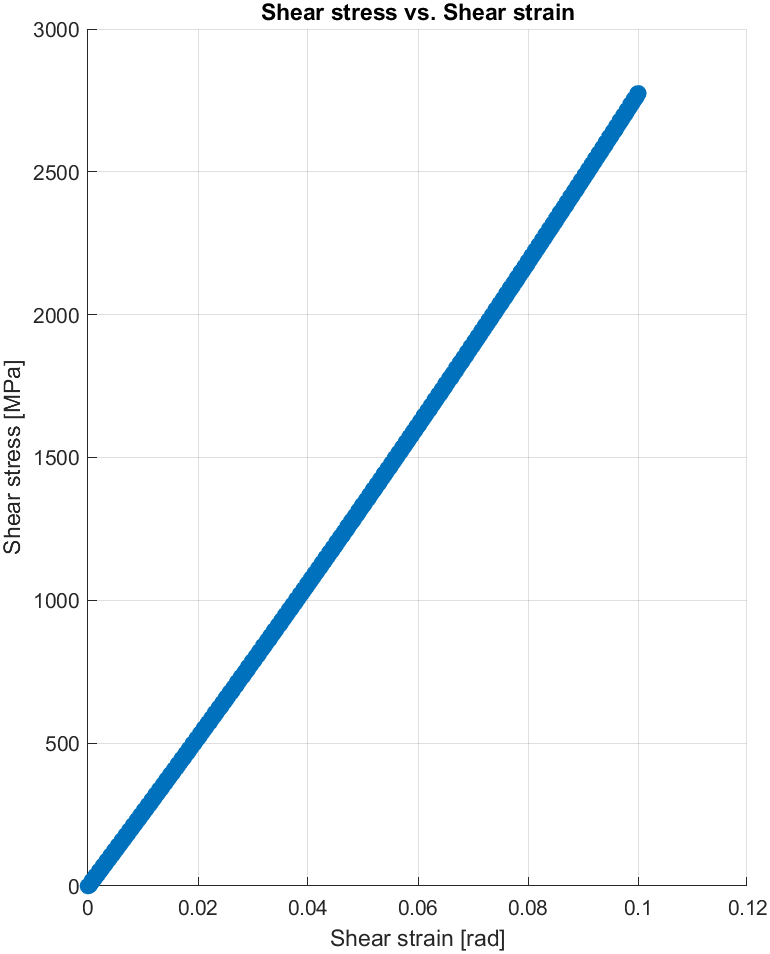
\includegraphics[width=\textwidth]{img/shear_stress_vs_strain.png}
        \caption{Average shear stress $\sigma_{12}$ as a function of the shear strain $\gamma$.}
        \label{fig:shear_stress_vs_strain}
    \end{minipage}
    %
    \hfill
    %
    \begin{minipage}[b]{0.45\textwidth}
        \centering
        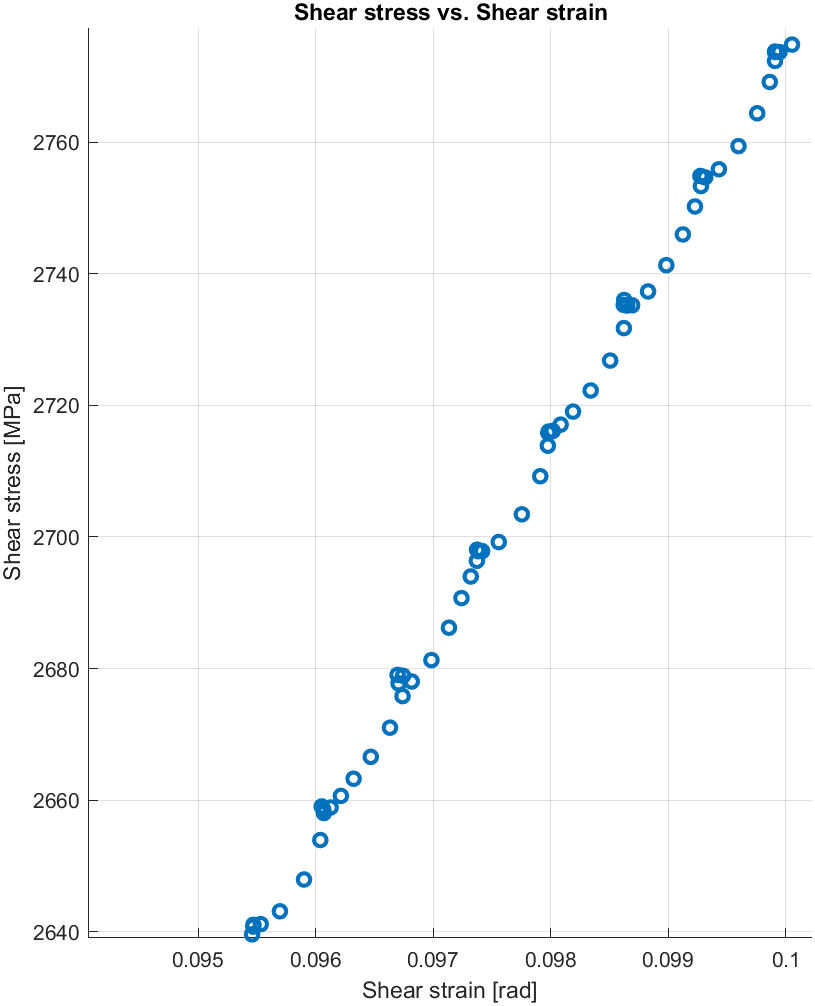
\includegraphics[width=\textwidth]{img/shear_stress_vs_strain_focus.png}
        \caption{Focus on the oscillation of the curve $\sigma_{12}(\gamma)$.}
        \label{fig:shear_stress_vs_strain_focus}
    \end{minipage}

\end{figure}

From the plot, it's clearly visible a general linear trend of the stress-strain curve, which is typical for a linear elastic material.
In particular, the curve well approximate the ideal behavior having a slope almost equal to the shear modulus $G = \frac{E}{2(1 + \nu)} = 26.923 \text{GPa}$, characteristic of the elastic region of the material.

However, because of the inertia effects and the high loading speed, the curve is not perfectly linear, and it shows some oscillations.
When the loading speed is reduced to a more realistic value, such as $v = 0.001 \text{m/s}$, the inertia effects are strongly reduced, and the oscillatory behavior of the curve is almost completely removed.


\paragraph{Initial and final positions of the structure}

In Figure \ref{fig:initial_vs_final}, we can observe the structure in both its initial configuration (shown in blue), and in its final configuration (shown in red).

\begin{figure}[H]
    \centering
    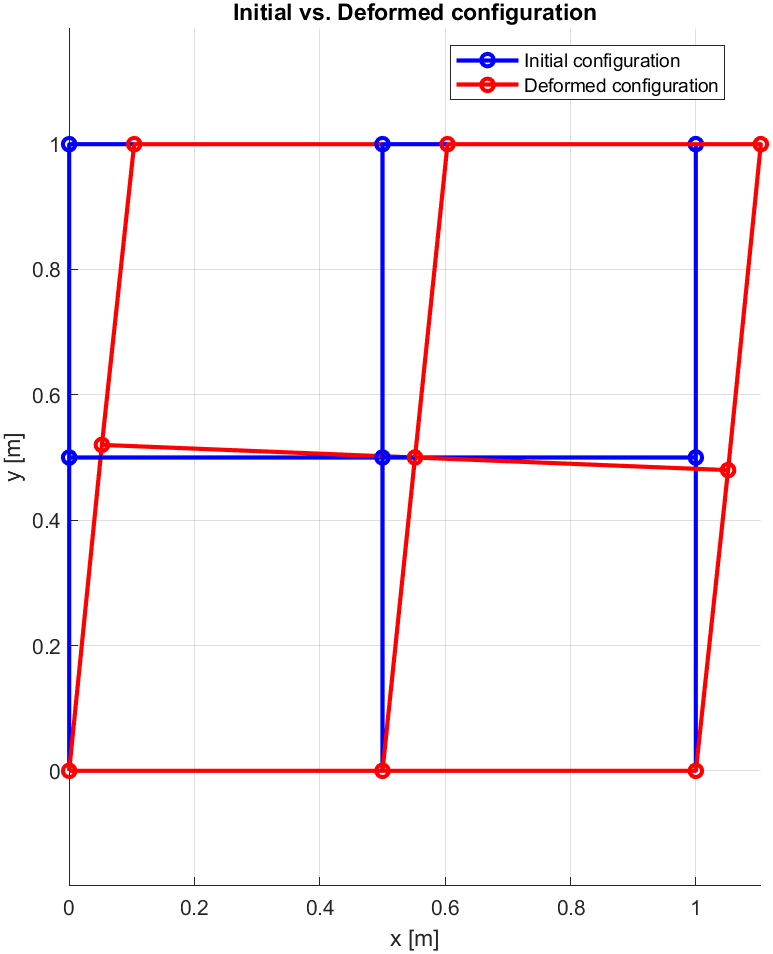
\includegraphics[width=0.5\textwidth]{img/initial_vs_final.png}
    \caption{Initial and final configurations of the structure.}
    \label{fig:initial_vs_final}
\end{figure}

The structure is deformed in the $\vec{x}$ direction, as expected, and the deformation is more pronounced in the top part of the structure where the velocity constrains is applied.
The deformation is almost linear, and the structure is not showing any sign of instability or excessive deformation.

The well known behavior of compression on the right side and tension on the left side of the lower half of the structure is clearly visible by observing the central line which is horizontal in the initial configuration and shows a clear clockwise rotation in the final configuration.


\paragraph{Computation time reduction}

Finally, a possible way to reduce the computation time when the loading speed is reduced to a more realistic value, such as $v = 0.001 \text{m/s}$, is to increase the density property of the material ($\rho$).

This choice is motivated by the fact that the time step of the simulation is usually limited by the smallest element of the mesh, which is the one that requires the smallest time step to satisfy convergence and stability conditions.
In particular:

\begin{equation}
    \Delta t = \frac{2}{\omega_{max}}
    \label{eq:time_step}
\end{equation}

where $\omega_{max}$ is the maximum frequency of the system, computable as the largest eigenvalues of the equation of motion for the element (i.e., $[M] \ddot{U} + [K] U = 0 \rightarrow det([M] \omega^2 - [K]) = 0 \rightarrow \omega_{max}$).
By solving the equation, we obtain the following expression for the time step:

\begin{equation}
    \Delta t = \frac{L_{min}}{c} = \frac{L_{min}}{\sqrt{\frac{E}{\rho}}} = \frac{L_{min}}{\sqrt{E}} \sqrt{\rho}
    \label{eq:time_step_2}
\end{equation}


where $L_{min}$ is the smallest characteristic length of the element, and $c$ is the speed of sound in the material.

From Equation \ref{eq:time_step_2}, it's clear that by increasing the density of the material, the time step of the simulation is increased as well, and the computation time is decreased.

One may wonder if the choice of increasing the density of the material may affect the results of the simulation.
For this purpose, we report in Table \ref{tab:time_step_validation} the results of the simulation for two different values of applied velocity $v_{top}$ and density $\rho$.

\begin{table}[H]
    \centering
    \begin{tabular}{|l|c|c|c|c|c|}
        \hline
        ~            & $v_{top}$ & $\rho$                  & CPU time & $U_x$  & $U_y$  \\
        ~            & m/s       & kg/m\textsuperscript{3} & s        & m      & m      \\
        \hline
        Simulation 1 & 1         & 2700                    & 9.64     & 0.5518 & 0.5000 \\
        Simulation 2 & 0.01      & 2700                    & 662.17   & 0.5518 & 0.5000 \\
        Simulation 3 & 0.01      & 27000000                & 7.68     & 0.5518 & 0.4992 \\
        \hline
    \end{tabular}
    \caption{
        Results of the simulation for different values of applied velocity $v_{top}$ and density $\rho$.
        Here $U_x$ and $U_y$ are the displacements of the central node of the structure.
        When increasing the density of the material, the external body force (gravity) is increased as well.
    }
    \label{tab:time_step_validation}
\end{table}

From Table \ref{tab:time_step_validation}, it's clear that the results of the simulation are not affected by the choice of increasing the density of the material (as long as the mesh is sufficiently fine) and that the computation time is significantly reduced by this choice.


\subsection{Effect of mesh refinement}

It's worth mentioning that the results of the simulation are affected by the choice of the mesh size.

In Figure \ref{fig:mesh_refinement}, we report the results of the simulation runned with same boundary conditions (Table \ref{tab:boundary_conditions_for_mesh_refinement}) but different mesh sizes (Table \ref{tab:mesh_sizes}).

\begin{table}[H]
    \centering
    \begin{tabular}{|l|c|c|c|c|}
        \hline
        ~            & $U_x$ & $U_y$ & $V_x$ & $V_y$ \\
        ~            & m     & m     & m/s   & m/s   \\
        \hline
        Bottom nodes & Fixed & Fixed & 0     & 0     \\
        Top nodes    & -     & Fixed & 1000  & 0     \\
        \hline
    \end{tabular}
    \caption{Boundary conditions imposed on the structure.}
    \label{tab:boundary_conditions_for_mesh_refinement}
\end{table}

\begin{table}[H]
    \centering
    \begin{tabular}{|c|c|c|}
        \hline
        \textbf{Mesh size} & \textbf{Number of elements} & \textbf{CPU time (s)} \\
        \hline
        Coarse             & 2x2                         & 0.20                  \\
        Fine               & 4x20                        & 8.58                  \\
        \hline
    \end{tabular}
    \caption{Mesh sizes and CPU time of the simulations.}
    \label{tab:mesh_sizes}
\end{table}

\begin{figure}[H]
    \centering

    \begin{minipage}[b]{0.45\textwidth}
        \centering
        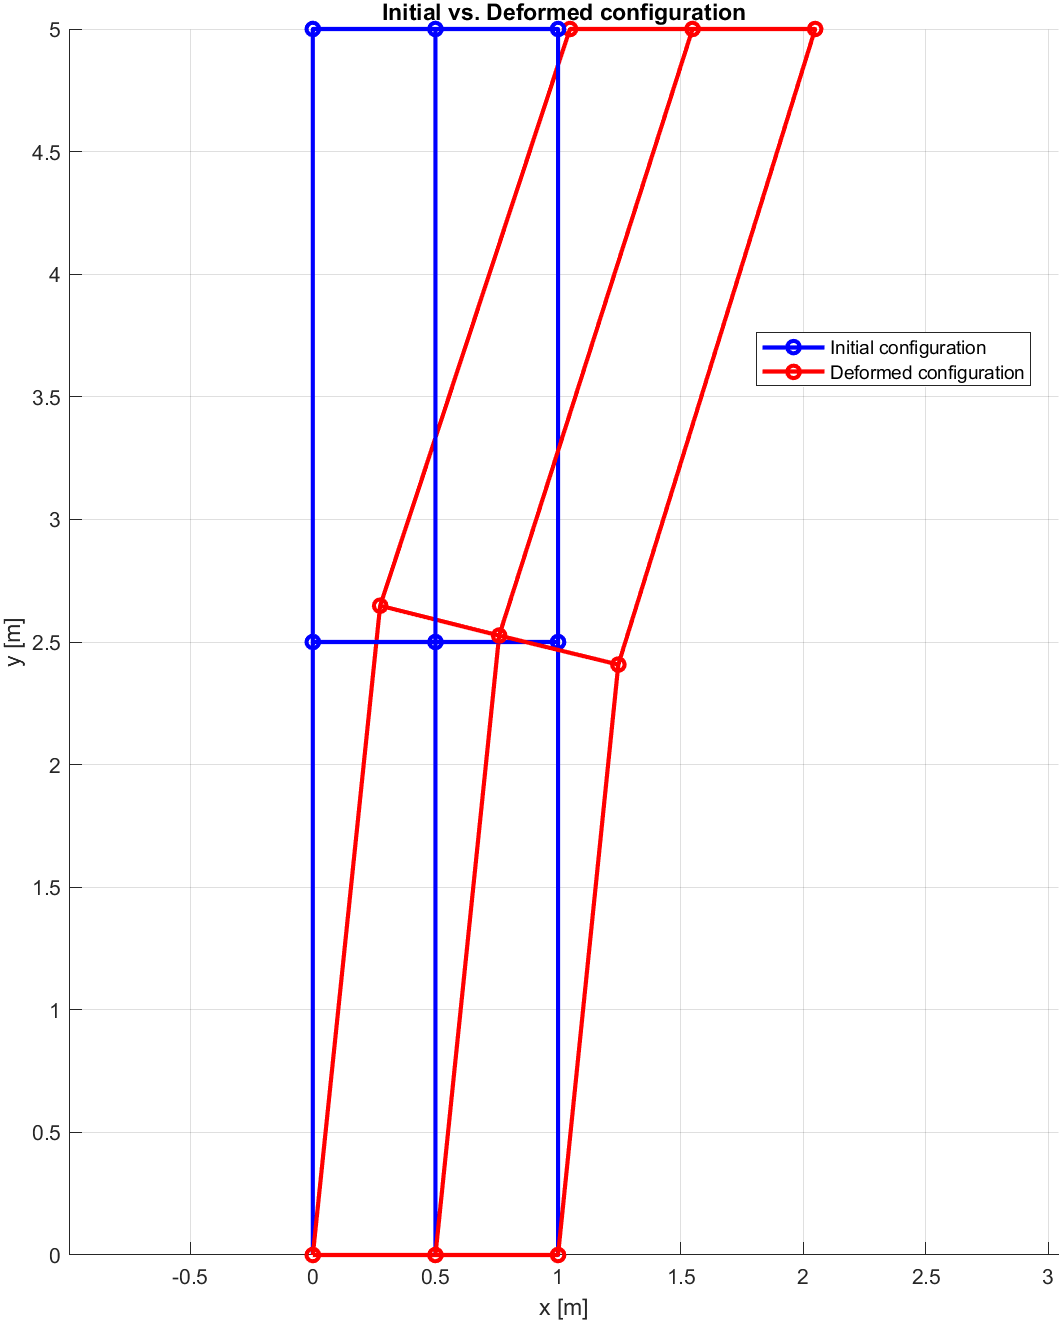
\includegraphics[width=\textwidth]{img/mesh_coarse.png}
        \caption{Coarse mesh.}
    \end{minipage}
    %
    \hfill
    %
    \begin{minipage}[b]{0.45\textwidth}
        \centering
        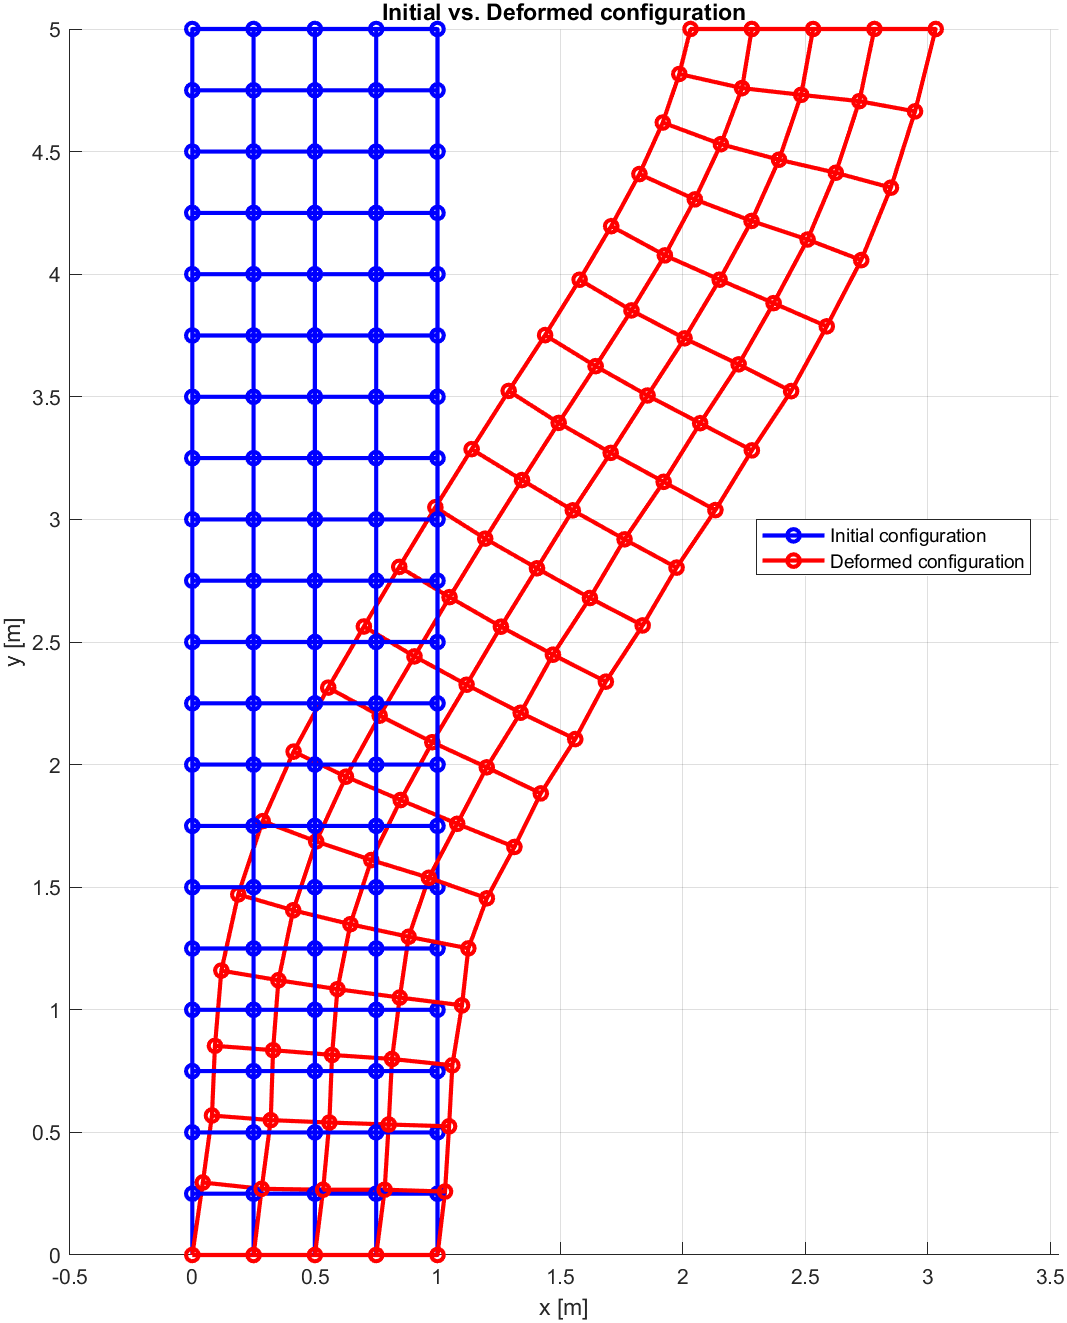
\includegraphics[width=\textwidth]{img/mesh_fine.png}
        \caption{Fine mesh.}
    \end{minipage}

    \caption{Effect of mesh refinement on the results of the simulation.}
    \label{fig:mesh_refinement}

\end{figure}

From Figure \ref{fig:mesh_refinement}, it's clear that the results of the simulation are affected by the choice of the mesh size.
In particular, given the high loading speed and the inertia effects, the results of the simulation are more accurate when a fine mesh is used, where the mass distribution is more accurate.
In the coarse mesh, the mass distribution is not accurate (on the central node an equivalent $25\%$ of the total mass is applied), and the inertia effects are not well represented, leading to a not realistic slow behavior of the node.


\clearpage
\appendix

\section{Flow Charts}
\label{appendix:flowcharts}

The following flow charts mimics the structure of the MATLAB code used to solve the problem.

The code is structured in three nested loops: the main loop (\textbf{Explicit Time Integration Algorithm}), the inner loop (\textbf{Stress Update Algorithm}) and the innermost loop (\textbf{Radial Return Algorithm}).

The Explicit Time Integration Algorithm is the main loop that iterates until the convergence criterion is met.
Inside the main loop, the Stress Update Algorithm is called to update the stress state of each element (at each integration point).

Inside the Stress Update Algorithm, the Radial Return Algorithm is called to update the stress state of each element (at each integration point) in case of plastic behavior.

\begin{figure}[H]
    \centering

    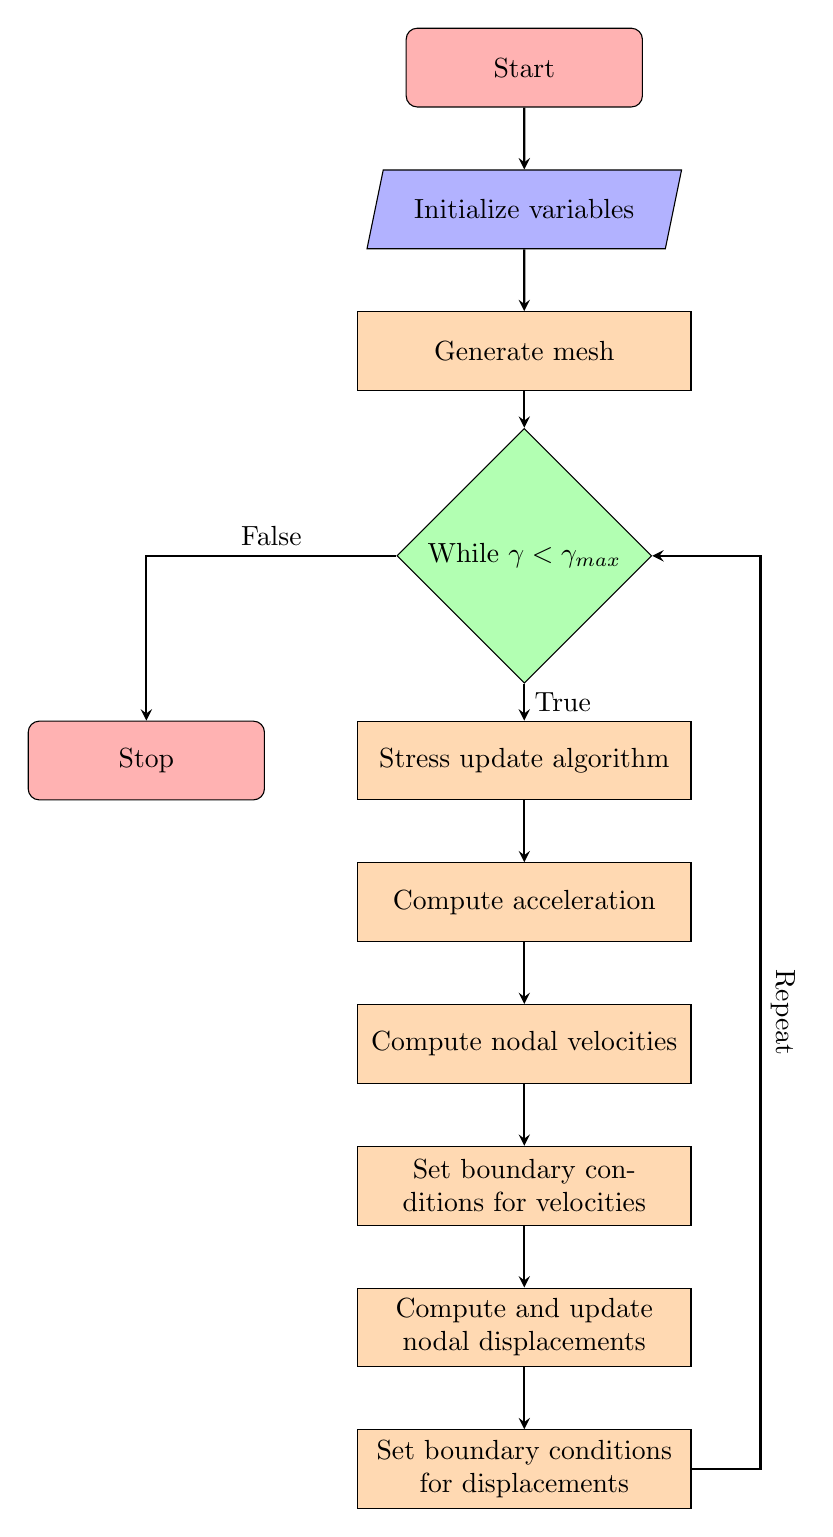
\begin{tikzpicture}[node distance=1.8cm]
        % Nodes
        \node (start) [startstop] {Start};
        \node (init) [io, below of=start] {Initialize variables};
        \node (mesh) [process, below of=init] {Generate mesh};

        \node (while) [decision, below of=mesh, yshift=-0.8cm] {While $\gamma < \gamma_{max}$};
        \node (stress) [process, below of=while, yshift=-0.8cm] {Stress update algorithm};
        \node (acceleration) [process, below of=stress] {Compute acceleration};
        \node (velocities) [process, below of=acceleration] {Compute nodal velocities};
        \node (enforce1) [process, below of=velocities] {Set boundary conditions for velocities};
        \node (update1) [process, below of=enforce1] {Compute and update nodal displacements};
        \node (enforce2) [process, below of=update1] {Set boundary conditions for displacements};
        \node (stop) [startstop, left of=stress, xshift=-3cm] {Stop};

        % Arrows
        \draw [arrow] (start) -- (init);
        \draw [arrow] (init) -- (mesh);
        \draw [arrow] (mesh) -- (while);
        \draw [arrow] (while) -- node[anchor=west] {True} (stress);
        \draw [arrow] (stress) -- (acceleration);
        \draw [arrow] (acceleration) -- (velocities);
        \draw [arrow] (velocities) -- (enforce1);
        \draw [arrow] (enforce1) -- (update1);
        \draw [arrow] (update1) -- (enforce2);
        \draw [arrow] (enforce2) -- +(3,0) |- (while.east) node[pos=0.25, above, rotate=-90] {Repeat};

        \draw [arrow] (while.west) -| node[pos=0.25, above] {False} (stop);
    \end{tikzpicture}

    \caption{
        Flowchart for the \textbf{Explicit Time Integration Algorithm}.
        The convergence criterion $\gamma < \gamma_{max}$ is relative to the given problem, while the rest of the algorithm is general.
    }
\end{figure}


\begin{figure}[H]
    \centering

    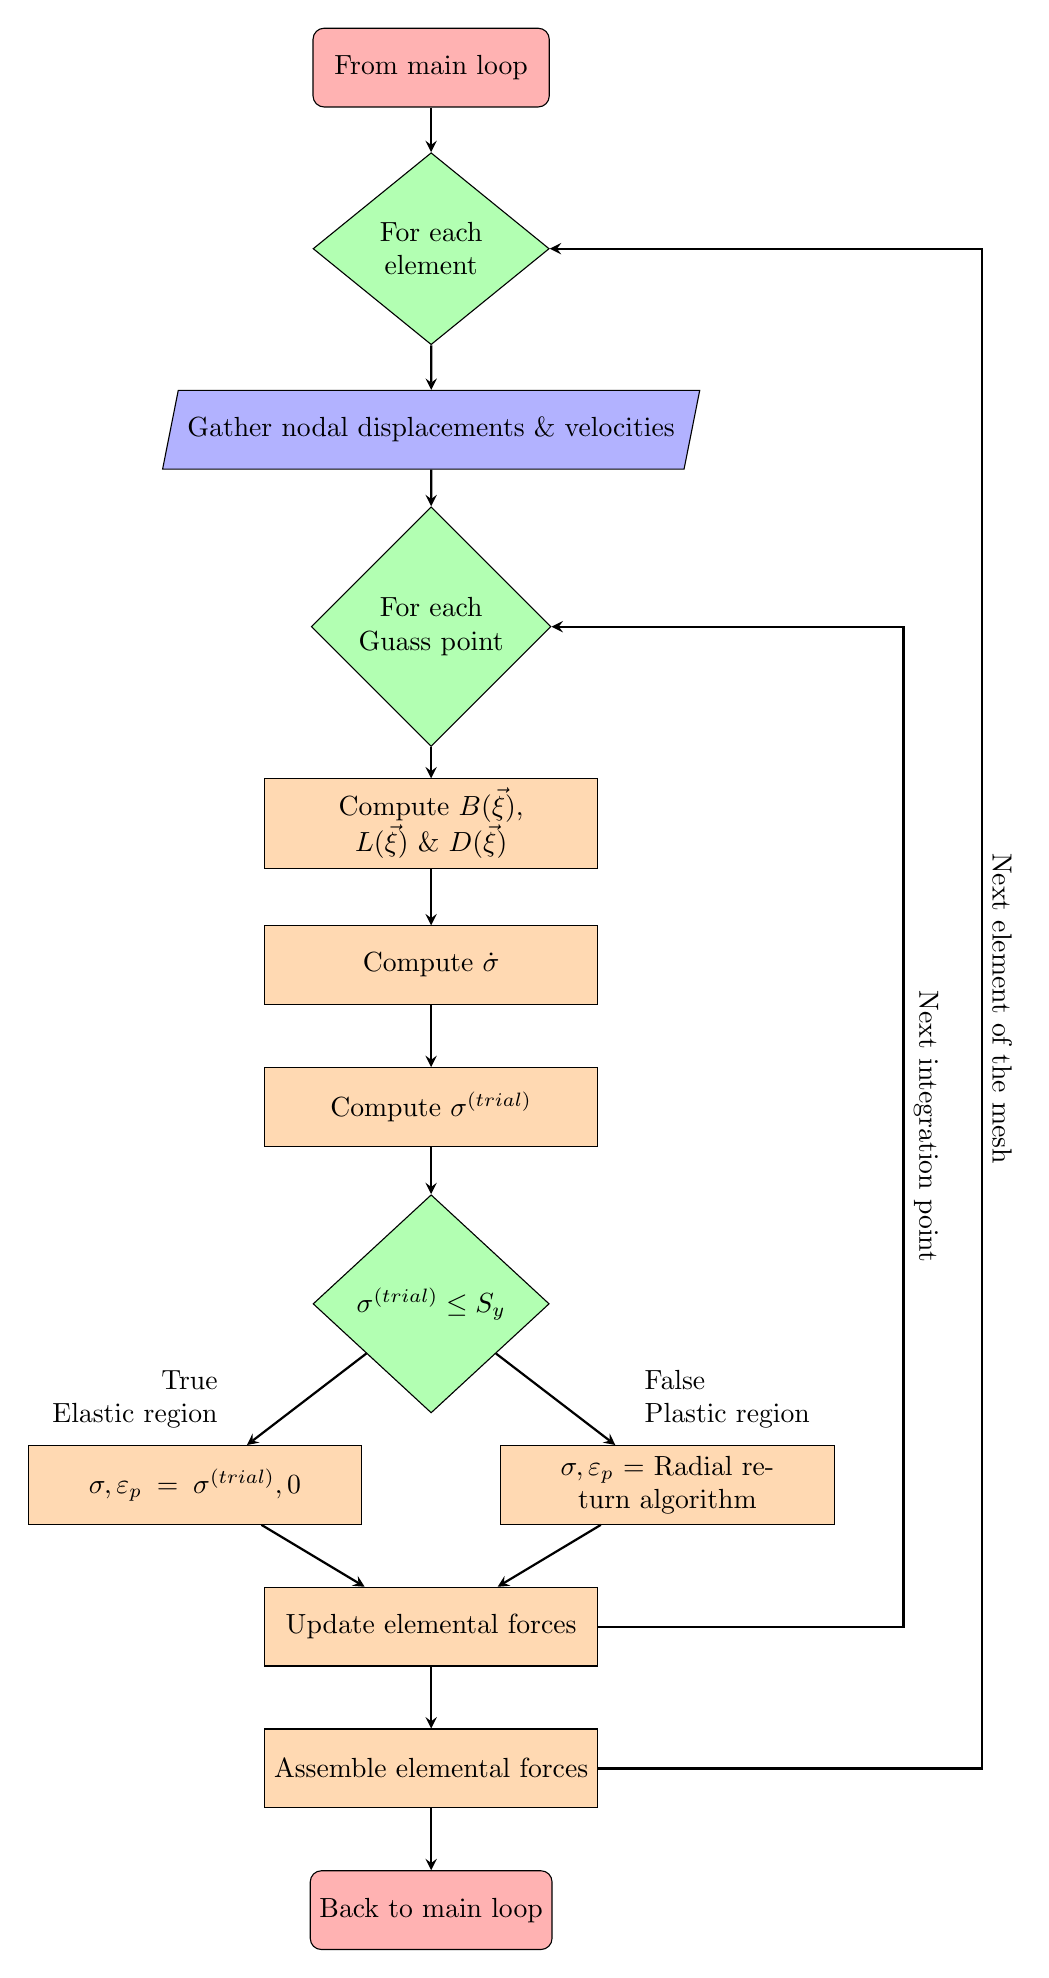
\begin{tikzpicture}[node distance=1.8cm]
        % Nodes
        \node (start) [startstop] {From main loop};
        \node (elementloop) [decision, below of=start, align=center, yshift=-0.5cm] {For each \\ element};
        \node (gather) [io, below of=elementloop, yshift=-0.5cm] {Gather nodal displacements \& velocities};

        \node (integrationloop) [decision, below of=gather, align=center, yshift=-0.7cm] {For each \\ Guass point};
        \node (computematrices) [process, below of=integrationloop, yshift=-0.7cm] {Compute $B(\vec{\xi})$, $L(\vec{\xi})$ \& $D(\vec{\xi})$};
        \node (compute) [process, below of=computematrices] {Compute $\dot{\sigma}$};
        \node (update) [process, below of=compute] {Compute $\sigma^{(trial)}$};
        \node (iselastic) [decision, below of=update, align=center, yshift=-0.7cm] {$\sigma^{(trial)} \le S_y$};
        \node (elastic) [process, below of=iselastic, yshift=-0.5cm, xshift=-3cm] {$\sigma, \varepsilon_p = \sigma^{(trial)}, 0$};
        \node (plastic) [process, below of=iselastic, yshift=-0.5cm, xshift=3cm] {$\sigma, \varepsilon_p$ = Radial return algorithm};

        \node (sumforces) [process, below of=elastic, xshift=3cm] {Update elemental forces};

        \node (scatter) [process, below of=sumforces] {Assemble elemental forces};
        \node (stop) [startstop, below of=scatter] {Back to main loop};

        % Arrows
        \draw [arrow] (start) -- (elementloop);
        \draw [arrow] (elementloop) -- (gather);
        \draw [arrow] (gather) -- (integrationloop);
        \draw [arrow] (integrationloop) -- (computematrices);
        \draw [arrow] (computematrices) -- (compute);
        \draw [arrow] (compute) -- (update);
        \draw [arrow] (update) -- (iselastic);
        \draw [arrow] (iselastic) -- node[anchor=east, xshift=-1cm, align=right] {True \\ Elastic region} (elastic);
        \draw [arrow] (iselastic) -- node[anchor=west, xshift=1cm, align=left] {False \\ Plastic region} (plastic);
        \draw [arrow] (elastic) -- (sumforces);
        \draw [arrow] (plastic) -- (sumforces);
        \draw [arrow] (sumforces) -- (scatter);
        \draw [arrow] (sumforces) -- +(6,0) |- (integrationloop.east) node[pos=0.25, above, rotate=-90] {Next integration point};
        \draw [arrow] (scatter) -- (stop);
        \draw [arrow] (scatter) -- +(7,0) |- (elementloop.east) node[pos=0.25, above, rotate=-90] {Next element of the mesh};

    \end{tikzpicture}

    \caption{
        Flowchart for the \textbf{Stress Update Algorithm}.
        The decision blocks in this case represent for loops over the elements and the integration points.
    }
\end{figure}


\begin{figure}[H]
    \centering

    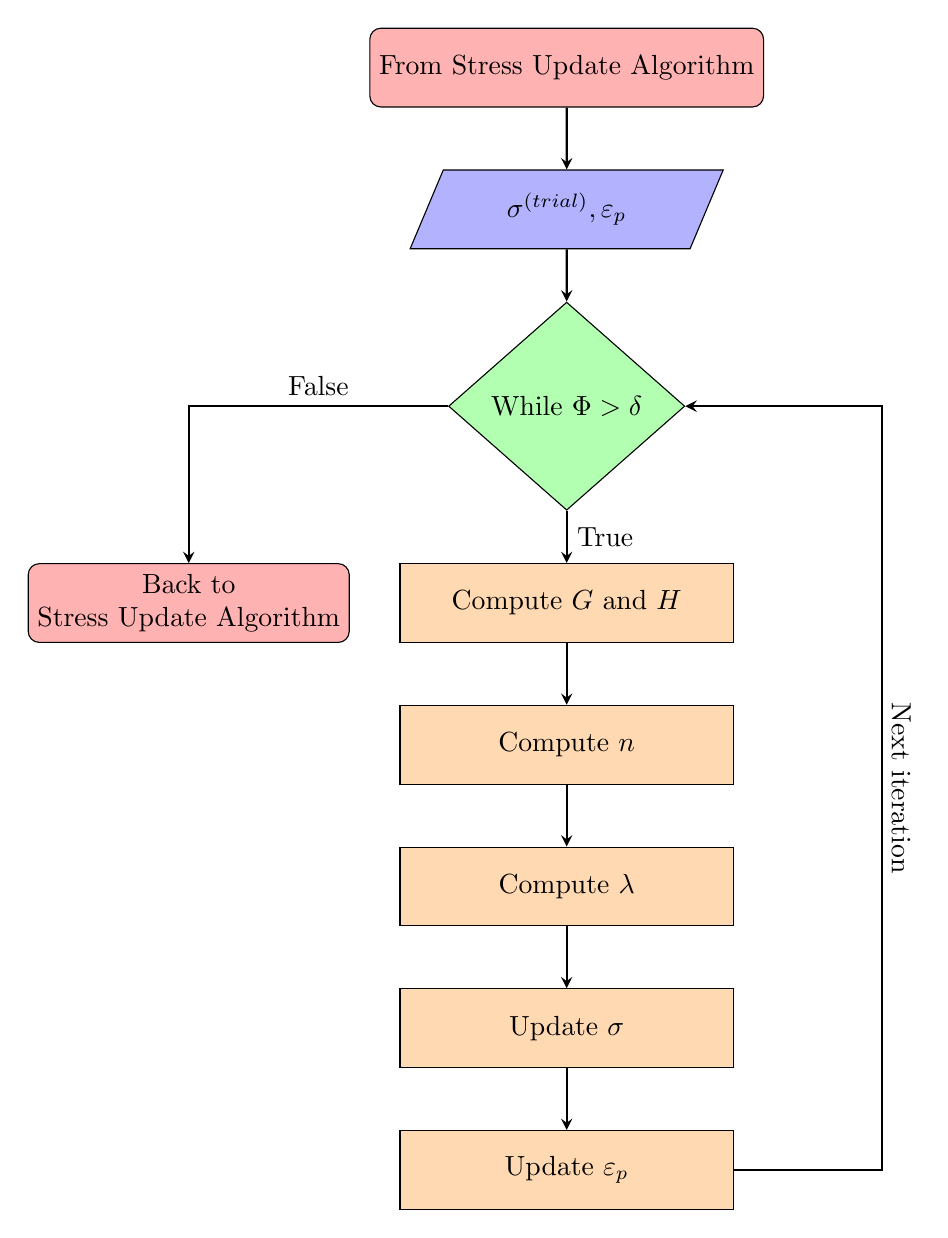
\begin{tikzpicture}[node distance=1.8cm]
        % Nodes
        \node (start) [startstop] {From Stress Update Algorithm};

        \node (init) [io, below of=start] {$\sigma^{(trial)}, \varepsilon_p$};

        \node (while) [decision, below of=init, yshift=-0.7cm] {While $\Phi > \delta$};

        \node (computeconstants) [process, below of=while, yshift=-0.7cm] {Compute $G$ and $H$};
        \node (computedirection) [process, below of=computeconstants] {Compute $n$};
        \node (computelambda) [process, below of=computedirection] {Compute $\lambda$};
        \node (updatestress) [process, below of=computelambda] {Update $\sigma$};
        \node (updateplastic) [process, below of=updatestress] {Update $\varepsilon_p$};

        \node (stop) [startstop, left of=computeconstants, xshift=-3cm, align=center] {Back to \\ Stress Update Algorithm};

        % Arrows
        \draw [arrow] (start) -- (init);
        \draw [arrow] (init) -- (while);
        \draw [arrow] (while) -- node[anchor=west] {True} (computeconstants);
        \draw [arrow] (computeconstants) -- (computedirection);
        \draw [arrow] (computedirection) -- (computelambda);
        \draw [arrow] (computelambda) -- (updatestress);
        \draw [arrow] (updatestress) -- (updateplastic);
        \draw [arrow] (updateplastic) -- +(4,0) |- (while.east) node[pos=0.25, above, rotate=-90] {Next iteration};

        \draw [arrow] (while.west) -| node[pos=0.25, above] {False} (stop);

    \end{tikzpicture}

    \caption{Flowchart for the \textbf{Radial Return Algorithm}.}
\end{figure}

\end{document}
